\section{Systematics and Uncertainties}
\label{sec:monoZ-syst}

Systematic uncertainties in the search include both theoretical and experimental sources.

For theoretical modelling uncertainties, the analysis follows as closely as possible the ATLAS Physics Modelling Group recommendations and prescriptions. The main components are listed below:
\begin{itemize}

\item The effect of renormalisation and factorisation scale variations ($\mu_R, \mu_F$) is evaluated using a three-point variation scheme, in which $\mu_R$ and $\mu_F$ are scaled simultaneously by factors of 2 and 1/2 to obtain the upward and downward variations, respectively. In general, both signal and background simulated samples provide internal event weights that are used to estimate these variations. The QCD scale uncertainties range from 4\% to 5\% in different signal samples.

\item Parton-shower and hadronisation uncertainties are evaluated using eigenvector variations of the \textsc{Pythia}~8 A14 tune, where available (e.g., for top-pair production). For signal and diboson samples generated with \textsc{Sherpa}, alternative truth-level samples are used. Typical parton-shower uncertainties range from 1\% to 4\% for different MC samples.

\item For the signal and $\text{ZZ}$ samples, dedicated corrections are applied to account for electroweak (EW) effects, as described in the corresponding sections. The uncertainty of the EW correction is about 2\%.

\item For top-quark processes, alternative samples are used to evaluate the effects of different MC generators on the hard-scattering process (e.g., \textsc{Powheg} vs.\ \textsc{MadGraph5\_aMC@NLO}) and on the parton-showering model (e.g., \textsc{Powheg}+\textsc{Pythia}~8 vs.\ \textsc{Powheg}+\textsc{Herwig}~7). The associated uncertainty is at the 1\% level.

\item The impact of parton distribution function (PDF) uncertainties is evaluated for both signal and background samples. The uncertainties range from 1\% to 2\%.

\end{itemize}

The experimental uncertainties include contributions from lepton reconstruction and identification, trigger efficiencies, and the energy/momentum scale and resolution. Systematic uncertainties related to jets, $E_{\text{T}}^{\text{miss}}$, flavour-tagging, pile-up, and luminosity are also considered. The impact of each major experimental systematic uncertainty on the signal is reported as ``up'' ($+1\sigma$) and ``down'' ($-1\sigma$) variations. Overall, the total experimental uncertainties remain below 2.5\% for all signal samples.

%%%%%%%%%%%%%%%%
For signal processes, Tables~\ref{tab:syst-uncertainties-ee} and~\ref{tab:syst-uncertainties-mm} show the impact of the experimental uncertainties on the $qq \to \text{ZH}$ signal in the $ee$ and $\mu\mu$ channels, respectively. Tables~\ref{tab:syst-uncertainties-MonoZ-ee} and~\ref{tab:syst-uncertainties-MonoZ-mm} summarize the individual impacts for the benchmark axial-vector signal in the $ee$ and $\mu\mu$ channels, respectively. The full mapping between the physical descriptions used in these tables and the specific ATLAS internal parameter names is provided in Appendix~\ref{subsec:app_syst}.

The systematic uncertainties on the total yield for all reconstructed simplified models and the 2HDM+$a$ model signals are shown in Figures~\ref{fig:MonoZ-syst}(a) and (b). Binned variations for each source are used in the limit-setting procedure.

%------------------------
\begin{table}[!htbp]
\centering
\begin{tabular}{lrr}
\toprule
\textbf{Systematic source} ($ee + E_{\text{T}}^{\text{miss}}$ channel) & \textbf{Up (\%)} & \textbf{Down (\%)} \\
\midrule
Jet flavour composition                         & $-1.29$ &  $1.17$ \\
Jet energy resolution (component 1)             &  $0.93$ & $-0.93$ \\
Jet pile-up ($\rho$ topology)                   & $-0.70$ &  $0.75$ \\
Jet pile-up ($\mu$ offset)                      & $-0.76$ &  $0.57$ \\
Pile-up reweighting                             & $-0.77$ &  $0.50$ \\
Jet $\eta$-intercalibration (modelling)         & $-0.71$ &  $0.57$ \\
Jet flavour response                            &  $0.52$ & $-0.41$ \\
Jet energy resolution (component 2)             &  $0.43$ & $-0.43$ \\
Electron identification (component 8)           &  $0.37$ & $-0.37$ \\
Jet energy resolution (component 4)             &  $0.36$ & $-0.36$ \\
Jet energy resolution (component 5)             &  $0.35$ & $-0.35$ \\
Jet energy scale modelling (component 1)        & $-0.30$ &  $0.38$ \\
Jet pile-up ($N_{\text{PV}}$ offset)            & $-0.34$ &  $0.33$ \\
Electron reconstruction efficiency              &  $0.33$ & $-0.33$ \\
Electron energy scale                           &  $0.31$ & $-0.32$ \\
Jet energy resolution (component 6)             &  $0.30$ & $-0.30$ \\
Light-jet tagging efficiency                    & $-0.29$ &  $0.29$ \\
Electron identification (component 17)          &  $0.27$ & $-0.27$ \\
Jet energy resolution (data vs MC)              &  $0.25$ & $-0.25$ \\
Jet energy resolution (rest term)               &  $0.24$ & $-0.24$ \\
\midrule
\textbf{Total} &$+2.57$ & $-2.36$ \\
\bottomrule
\end{tabular}
\caption{\rm Impact of the 20 dominant experimental uncertainties on the $qq \to \text{ZH}$ signal in the $ee$ channel. The total positive (negative) uncertainty is calculated by summing the largest positive (negative) variations for each source in quadrature, including smaller sources that are not shown.}
\label{tab:syst-uncertainties-ee}
\end{table}

%%%%%%%%%%%%%%%%
\begin{table}[!htbp]
\centering
\begin{tabular}{lrr}
\toprule
\textbf{Systematic source} ($\mu\mu + E_{\text{T}}^{\text{miss}}$ channel) & \textbf{Up (\%)} & \textbf{Down (\%)} \\
\midrule
Jet flavour composition                         & $-1.23$ &  $1.04$ \\
Jet energy resolution (component 1)             &  $0.92$ & $-0.92$ \\
Jet $\eta$-intercalibration (modelling)         & $-0.73$ &  $0.58$ \\
Jet pile-up ($\rho$ topology)                   & $-0.68$ &  $0.64$ \\
Jet pile-up ($\mu$ offset)                      & $-0.65$ &  $0.50$ \\
Muon reconstruction efficiency (syst.)          &  $0.51$ & $-0.50$ \\                                
Jet flavour response                            &  $0.42$ & $-0.44$ \\
Pile-up reweighting                             & $-0.29$ &  $0.50$ \\
Jet energy resolution (component 2)             &  $0.39$ & $-0.39$ \\ 
Muon isolation efficiency (syst.)               &  $0.39$ & $-0.36$ \\
Muon isolation efficiency (stat.)               &  $0.36$ & $-0.36$ \\
Jet energy scale modelling (component 1)        &  $0.34$ &  $0.30$ \\
Jet pile-up ($N_{\text{PV}}$ offset)            & $-0.31$ &  $0.29$ \\
Jet energy resolution (component 6)             &  $0.30$ & $-0.30$ \\
Light-jet tagging efficiency                    & $-0.29$ &  $0.29$ \\
$E_{\text{T}}^{\text{miss}}$ soft-track resolution (para.) & $-0.27$ & $-0.27$ \\
Jet energy resolution (component 4)             &  $0.26$ & $-0.26$ \\
Jet energy resolution (rest term)               &  $0.25$ & $-0.25$ \\
Jet energy resolution (component 3)             &  $0.25$ & $-0.25$ \\
Jet energy resolution (component 5)             &  $0.25$ & $-0.25$ \\
\midrule
\textbf{Total}  & $+2.37$ & $-2.21$ \\
\bottomrule
\end{tabular}
\caption{\rm Impact of the 20 dominant experimental uncertainties on the $qq \to \text{ZH}$ signal in the $\mu\mu$ channel. The total positive (negative) uncertainty is calculated by summing the largest positive (negative) variations for each source in quadrature, including smaller sources that are not shown.}
\label{tab:syst-uncertainties-mm}
\end{table}
%%%%%%%%%%%%%%%%

\begin{table}[!htbp]
\centering
\begin{tabular}{lrr}
\toprule
\textbf{Systematic source} ($ee + E_{\text{T}}^{\text{miss}}$ channel) & \textbf{Up (\%)} & \textbf{Down (\%)} \\
\midrule
Electron identification (component 8)           & $+1.06$ & $-1.06$ \\
Jet flavour composition                         & $-0.81$ & $+0.91$ \\
Jet energy resolution (component 1)             & $+0.60$ & $-0.60$ \\
Pile-up reweighting                             & $-0.55$ & $+0.49$ \\
Electron identification (component 17)          & $+0.53$ & $-0.53$ \\
Jet pile-up ($\rho$ topology)                   & $-0.46$ & $+0.48$ \\
Jet pile-up ($\mu$ offset)                      & $-0.47$ & $+0.43$ \\
Jet $\eta$-intercalibration (modelling)         & $-0.45$ & $+0.40$ \\
Light-jet tagging efficiency                    & $-0.42$ & $+0.42$ \\
Electron reconstruction efficiency              & $+0.40$ & $-0.40$ \\
Electron identification (component 11)          & $+0.30$ & $-0.30$ \\
Jet flavour response                            & $+0.24$ & $-0.27$ \\
Electron energy scale                           & $+0.25$ & $-0.17$ \\
Jet energy resolution (component 2)             & $+0.19$ & $-0.19$ \\
Electron identification (component 13)          & $+0.19$ & $-0.19$ \\
Jet pile-up ($N_{\text{PV}}$ offset)            & $-0.15$ & $+0.17$ \\
Electron identification (component 10)          & $-0.17$ & $+0.17$ \\
Jet energy scale modelling (component 1)        & $-0.13$ & $+0.16$ \\
Jet energy resolution (component 3)             & $+0.16$ & $-0.16$ \\
Electron identification (component 15)          & $-0.15$ & $+0.15$ \\    
\midrule
\textbf{Total} & $+2.08$ & $-2.04$ \\ 
\bottomrule
\end{tabular}
\caption{\rm Impact of the 20 dominant experimental uncertainties on the Mono-$\text{Z}$ axial-vector $(m_\chi, m_{\text{med}}) = (1, 500)~\text{GeV}$ signal sample in the $ee$ channel. The total positive (negative) uncertainty is calculated by summing the largest positive (negative) variations for each source in quadrature, including smaller sources that are not shown.}
\label{tab:syst-uncertainties-MonoZ-ee}
\end{table}
%%%%%%%%%%%%%%%%%%%%%

\begin{table}[!htbp]
\centering
\begin{tabular}{lrr}
\toprule
\textbf{Systematic source} ($\mu\mu + E_{\text{T}}^{\text{miss}}$ channel) & \textbf{Up (\%)} & \textbf{Down (\%)} \\
\midrule
Jet flavour composition                         & $-0.89$ & $+0.77$ \\
Jet energy resolution (component 1)             & $+0.60$ & $-0.60$ \\
Muon reconstruction efficiency (syst.)          & $+0.59$ & $-0.59$ \\
Pile-up reweighting                             & $-0.58$ & $+0.51$ \\
Jet pile-up ($\rho$ topology)                   & $-0.47$ & $+0.44$ \\
Light-jet tagging efficiency                    & $-0.43$ & $+0.43$ \\
Jet pile-up ($\mu$ offset)                      & $-0.42$ & $+0.24$ \\
Jet $\eta$-intercalibration (modelling)         & $-0.34$ & $+0.39$ \\
Muon isolation efficiency (syst.)               & $+0.33$ & $-0.34$ \\
Muon isolation efficiency (stat.)               & $+0.33$ & $-0.33$ \\
Jet pile-up ($N_{\text{PV}}$ offset)            & $-0.26$ &  $0.00$ \\
Jet flavour response                            & $+0.24$ & $-0.21$ \\
Muon trigger efficiency (syst.)                 & $-0.21$ & $+0.21$ \\
Muon momentum scale (sagitta bias)              & $-0.10$ & $-0.21$ \\
Muon momentum scale (sagitta $\rho$)            & $-0.20$ & $-0.20$ \\
Jet energy resolution (component 4)             & $+0.18$ & $-0.18$ \\
Jet energy scale modelling (component 1)        & $-0.13$ & $+0.16$ \\
Muon identification efficiency                  & $-0.05$ & $-0.13$ \\
Muon track-to-vertex assoc. efficiency (syst.)  & $+0.11$ & $-0.10$ \\
Muon reconstruction efficiency (stat.)          & $+0.10$ & $-0.10$ \\
\midrule
\textbf{Total} & $+1.62$ & $-1.78$ \\    
\bottomrule
\end{tabular}
\caption{\rm Impact of the 20 dominant experimental uncertainties on the Mono-$\text{Z}$ axial-vector $(m_\chi, m_{\text{med}}) = (1, 500)~\text{GeV}$ signal sample in the $\mu\mu$ channel. The total positive (negative) uncertainty is calculated by summing the largest positive (negative) variations for each source in quadrature, including smaller sources that are not shown.}
\label{tab:syst-uncertainties-MonoZ-mm}
\end{table}
%%%%%%%%%%%%%%%%%%%%

\begin{figure}[!htbp]
    \centering
    \subfloat[]{
    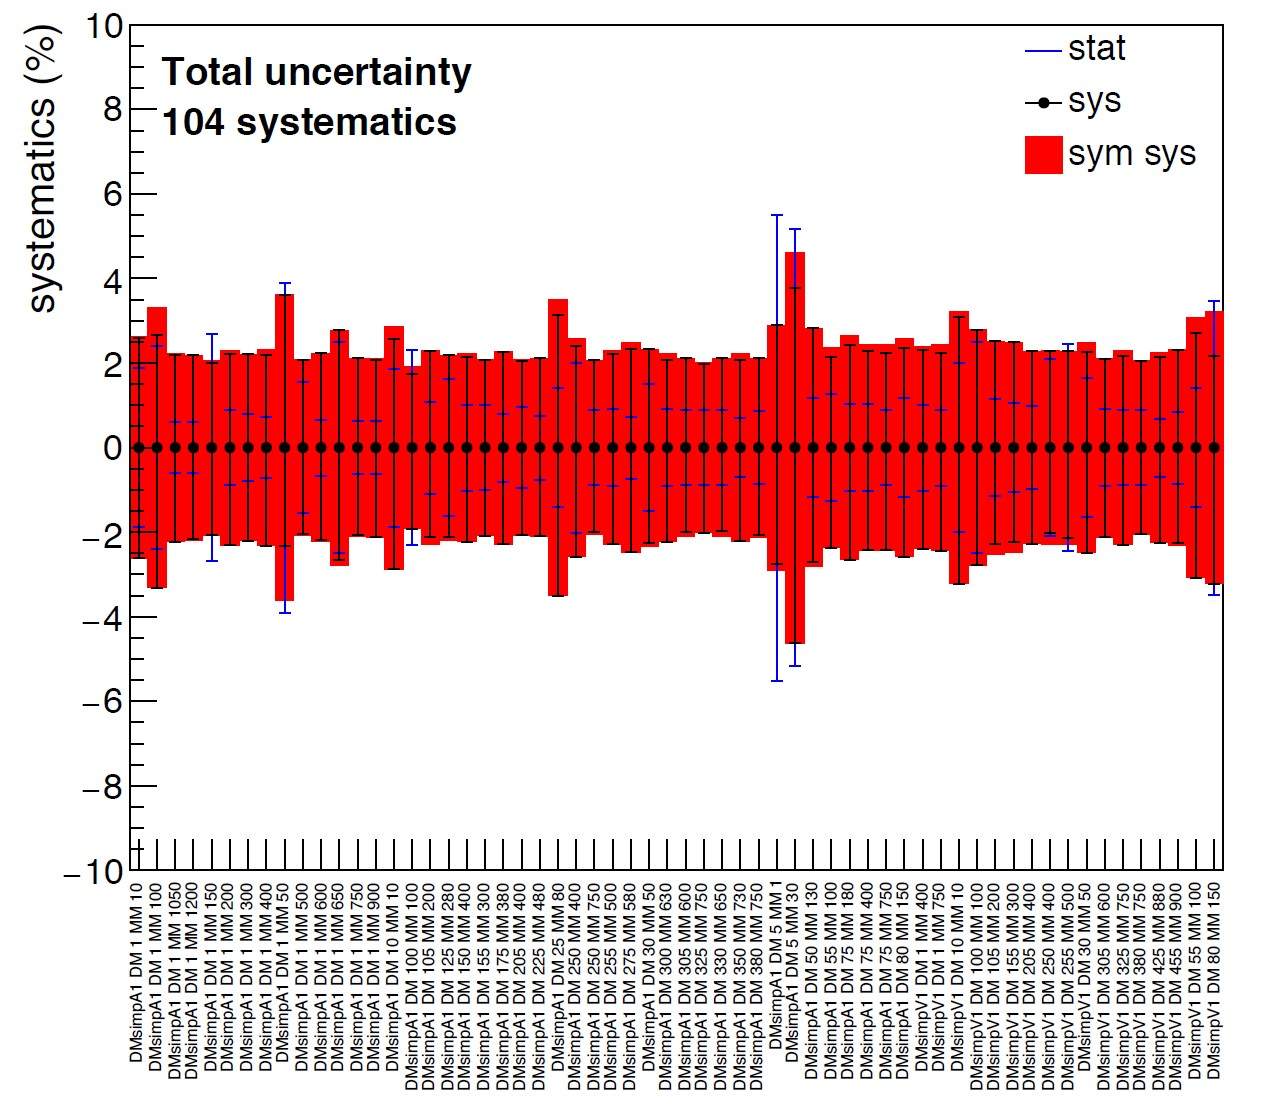
\includegraphics[width=0.8\linewidth]{figures/ch6-DM/ZHinv-syst-simplified-model.jpg}}\\
     \subfloat[]{
    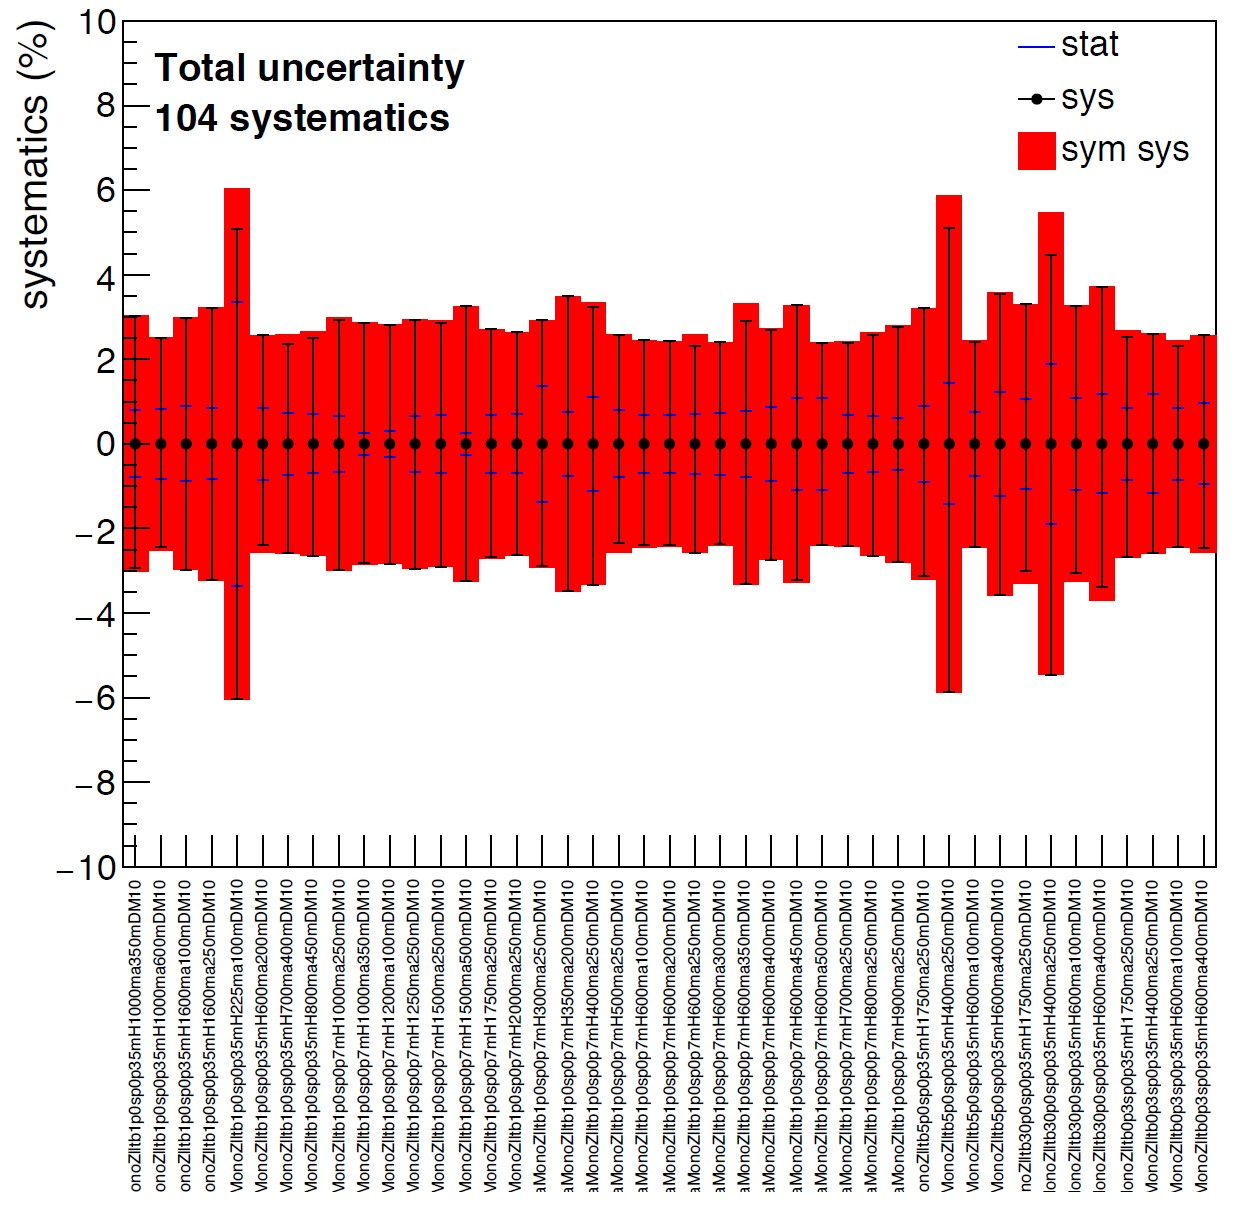
\includegraphics[width=0.8\linewidth]{figures/ch6-DM/ZHinv-syst-2HDMa.jpg}}
    \caption{\rm Summary of experimental uncertainties for all Mono-$\text{Z}$ (a) simplified model signal samples, and (b) 2HDM+$a$ samples.}
    \label{fig:MonoZ-syst}
\end{figure}

For some non-dominant backgrounds in the control regions (CRs), systematic uncertainties are assigned based on those evaluated in the signal region (SR). Specifically, normalization uncertainties on $\text{Z}$+jets are set to 38\% in the $e\mu$ and $3\ell$ CRs, while $\text{WZ}$ uncertainties in the $e\mu$ region are set to 9\%. The $\text{ZZ} \to \ell\ell\nu\nu$ uncertainties in the $e\mu$ and $3\ell$ CRs are set to 6.6\%, and 8.8\% for $\text{ZZ} \to 4\ell$. The uncertainties for the non-resonant processes in the $3\ell$ CR are set to 14\%. For triboson and $t\bar{t}\text{V}$ processes, conservative uncertainties of 50\% and 20\% are assumed, respectively.